\documentclass{article}
\usepackage{amsmath}
\usepackage{float}
\usepackage{graphicx}
\usepackage{listings}
\usepackage{amsmath}
\usepackage{lmodern}
\usepackage[left=2cm,right=2cm,
    top=2cm,bottom=2cm,bindingoffset=0cm]{geometry}
\usepackage{hyperref}
\usepackage[utf8]{inputenc}
\usepackage[russian]{babel}
\usepackage{indentfirst}
\usepackage{titlesec}
\setlength{\parindent}{4em}
\setlength{\parskip}{1em}
\titleformat*{\section}{\large\bfseries}
\titlespacing*{\section}
{0pt}{0ex}{0ex}
\begin{document}
\section*{Цель работы}
Целью работы является овладение методологией решения логических задач
с применением известных на сегодняшний день стратегий поиска в
пространстве состояний.
\section*{Задание 1}
Изучить на примере задачи о волке, козе и капусте работу базовой
программы для решения задач методом поиска в глубину. Задача имеет
следующий сюжет: \\
<<Однажды крестьянину понадобилось перевезти через реку волка, козу и
капусту. У крестьянина есть лодка, в которой может поместиться, кроме
самого крестьянина, только один объект — или волк, или коза, или
капуста. Если крестьянин оставит без присмотра волка с козой, то волк
съест козу; если крестьянин оставит без присмотра козу с капустой,
коза съест капусту. Как крестьянину перевезти на другой берег всё своё
имущество в целости и сохранности?>>
\section*{Результат выполнения задания 1}
В [1, с. 49] представлен код базовой программы для решения задач
поиска на графах состояний, который реализует алгоритм для решения
задачи о волке, козе и капусте. Код был адаптирован для интерпретатора
языка Prolog SWI-Prolog. Полный листинг новой версии программы представлен в
Приложении А.

Новая версия версия содержит следующие предикаты: solve\_dfs,
test\_dfs, initial\_tate, final\_state, move, update, update\_boat,
select, prededes, insert, update\_banks, legal и illegal.
Предикат solve\_dfs осуществляет решение головоломки путем обхода в
глубину. Предикат имеет два аргумента: первый аргумент ---
текущее состояние, включающее местоположение волка, козы, капусты и
лодки; второй аргумент --- история изменений состояния, третий
аргумент --- список сделанных шагов.

Предикат test\_dfs используется для более удобного извлечения решения
головоломки пользователем, чем с помощью предиката
solve\_dfs. Предикат имеет всего два аргумента: первый аргумент ---
исходное состояние задачи, второй аргумент --- список сделанных шагов.

Предикат initial\_state задает исходное состояние задачи. Он имеет два
аргумента: первый аргумент --- описание исходного состояния, второй
аргумент --- само состояние задачи.

Предикат final\_state задает конечное состояние задачи. Он имеет лишь
один аргумент --- состояние задачи.

Предикат move определяет допустимые шаги для определенного состояния. Он имеет два аргумента --- состояние задачи и сам шаг.

Предикат update обновляет состояние задачи в зависимости от данного
шага. Он имеет три аргумента: первый аргумент --- изначальное
состояние, второй аргумент --- шаг, третий аргумент --- получившееся в
результате выполнения шага состояния.

Предикат update\_boat <<переводит>> лодку с одного берега на
другой. Он имеет два аргумента --- местонахождение лодки до того, как
она переплыла на противоположный берег, и местонахождение лодки после.

Предикат select <<увозит>> обитателя с определенного
берега. Он имеет три аргумента: первый аргумент --- волк, коза или
капуста, второй аргумент --- список обитателей на береге до
осуществления действия, третий аргумент --- список обитателей берега после.

Предикат precedes определяет порядок сортировки обитателей на
береге. Для того, чтобы избежать циклов при решении задачи
(последовательности действий, приводящих к тому же самому состоянию),
при добавлении обитателя в список обитателей берега он добавляется в
список таким образом, чтобы список обитателей оставался
отсортированным. Предикат состоит из двух фактов:
<<precedes('Волк',\_).>> (т.е. <<волк всегда первый в списке
обитателей берега>>) и <<precedes(\_,'Капуста')>> (т.е. <<капуста
всегда последняя>>).

Предикат insert вставляет обитателя в список обитателей берега. Он
имеет три аргумента: первый аргумент --- новый обитатель берега,
второй аргумент --- исходный список обитателей, третий аргумент ---
модифицированный список обитателей.

Предикат update\_banks <<перевозит>> обиталея с одного берега на
противоположный. Он имеет три аргумента: первый аргумент ---
перевозимый обитатель, второй аргумент --- местонахождение лодки,
третий аргумент --- список обитателей левого берега до перевозки,
четверый аргумент --- список обитателей правого берега до перевозки,
пятый аргумент --- список обитателей левого берега после перевозки,
шестой аргумент --- список обитателей правого берега после перевозки.

Предикат legal определяет, допустимо ли определенное состояние
задачи. Состояние является недопустимым, если волк и коза, либо
капуста и коза остались одни без присмотра крестьянина.

Предикат illegal определяет недопустимые состояния задачи.

\section*{Задание 2}
Написать программу для решения задачи о двух кувшинах. Формулировка
задачи: Дан кувшин с водой емкостью N и пустой кувшин емкостью
M. Требуется получить заданную емкость L. Воду можно либо выливать,
либо переливать из одного кувшина в другой. (Kувшины можно полностью
наполнять водой из неогpаниченного pезеpвуаpа). 
\section*{Результат выполнения задания 2}
Была разработана программа для решения задачи о двух
кувшинках. Листинг программы представлен в Приложении А. Программа
состоит из предикатов final\_state, move, update, solve\_dfs и
test\_dfs.

Предикат final\_state определяет итоговое состояние задачи --- в одной
из двух кувшинках находится объем воды L.

Предикат move аналогичен предикату move из Задания 1, он определяет
возможные ходы для определенного состояния.

Предикат update аналогичен предикату update из Задания 1, он меняет
текущее состояние задачи в зависимости от определенного хода.

Предикат solve\_dfs аналогичен предикату solve\_dfs из Задания 1. Он
производит поиск решения путем обхода в глубину.

Предикат test\_dfs аналогичен предикату test\_dfs из Задания 1, он
используется для получения решения головоломки. Он имеет следующие
аргументы: первый аргумент --- объем L, второй аргумент --- объем N,
третий аргумент --- объем M, четвертый аргумент --- искомая
последовательность шагов.

\section*{Задание 3}
Написать программу для нахождения решения Игры в восемь. Целевая конфигурация представлена на рисунке 1. Правила игры следующие:\\
<<На игровом поле 3 на 3 расставлены фишки с цифрами от 1 до
8. Имеется одна свободная клетка, на которую могут быть передвинуты
фишки с соседних позиций. При этом не допускается перемещение фишек
через одну, а также по диагонали. Задача состоит в том, чтобы
преобразовать некоторую начальную конфигурацию в целевую
конфигурацию.>>
\begin{figure}[H]
  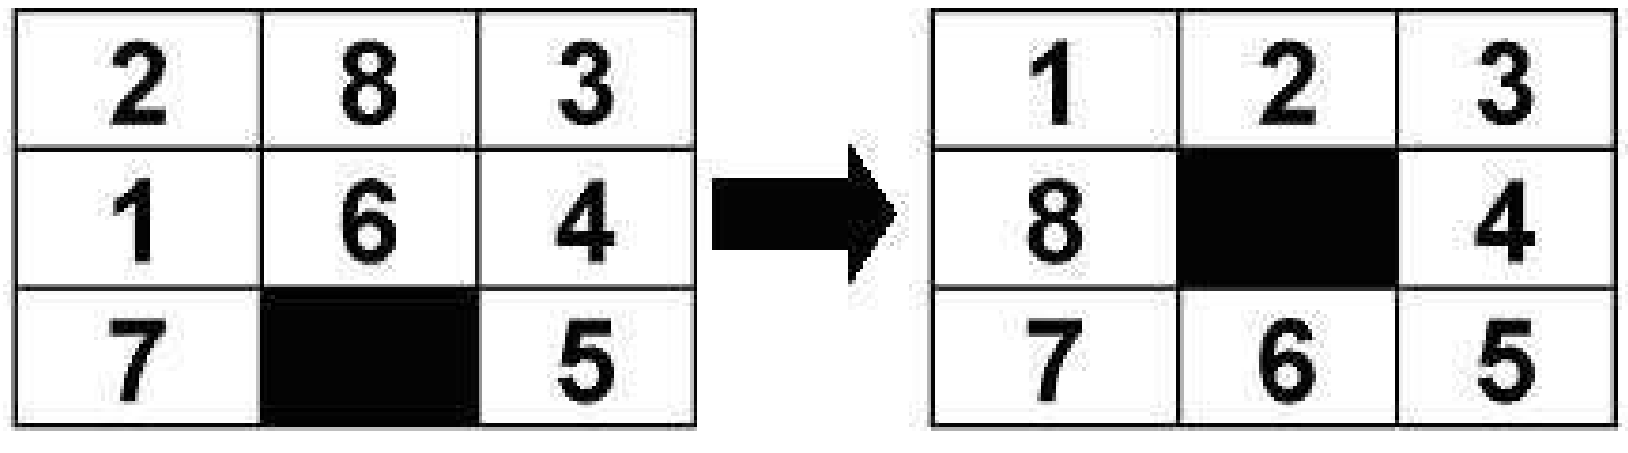
\includegraphics[width=\linewidth]{puzzle.png}
  \caption{Пример начальной и целевая конфигурация для игры в восемь}
  \label{fig:puzzle}
\end{figure}
\section*{Результат выполнения задания 3}
Была разработана программа для нахождения решения Игры в восемь в
зависимости от введенной начальной конфигурации. Листинг программы
представлен в Приложении А. Программа состоит из следующих предикатов:
move, moveRow, moveCol, final\_state, updateRow, update, mapetop, h,
findPos, heu, f\_func, solve, search, expand, insert\_all, repMode,
insert, cheaper, solvable, countGT, countInv, solver.

Предикат move определяет допустимость шага для определенной
конфигурации. Всего существует четыре шага: moveUp --- передвинуть
фишку вниз, moveLeft --- передвинуть фишку вправо, moveRight ---
передвинуть фишку влево, moveDown --- передвинуть фишку вверх. Такое
название шагов связано с тем, что при решении задачи удобнее
представлять, что по доске передвигается не фишка, а пустое место, при
этом пустое место передвигается в противоположном направлении тому
направлению, по которому передвигается фишка. Предикат имеет следующие
аргументы: первый аргумент --- текущая конфигурация доски, второй
аргумент --- шаг. Конфигурация доски в программе представляется как
список. Например, для целевой конфигурации (см. рис. 1) ее
представление в программе будет выглядеть следующим образом:
[[1,2,3],[8,0,4],[7,6,5]]. Пустое место на доске представляется в программе как 0.

Предикат moveRow определяет возможный для строки доски
(т.е. горизонтальной линии клеток) ход. Например, если одна из
строк доски выглядит так --- <<[0,1,2]>>, то фишку <<1>> можно
передвинуть влево. Предикат имеет два аргумента --- строку доски и
движение.

Предикат moveCol определяет возможный для столбца доски
(т.е. вертикальной линии клеток) ход, если бы столбец доски можно было
представить в виде строки доски. Например, если представить столбец в
виде строки <<[X,Y,Z]>>, где X --- первая клетка первой строки, Y ---
первая клетка второй строки, Z --- первая клетка третьей строки, то
движение <<moveUp>> будет соответствовать движению <<moveLeft>>, а
движение <<moveDown>> будет соответствовать движению <<moveRight>>.

Предикат final\_state определяет целевую конфигурацию.

Предикат update\_row изменяет состояние строки доски в зависимости от
движения. Предикат имеет три аргумента: первый аргумент --- входная
строка, второй аргумент --- движение, третий аргумент --- выходная
строка.

Предикат update изменяет конфигурацию доски в зависимости от
движения. Предикат имеет три аргумента: первый аргумент --- входная
конфигурация доски, второй аргумент --- движение, третий аргумент ---
выходная конфигурация доски.

Предикат mapetop определяет номер столбца и номер строки доски, где
находится фишка с точки зрения целевой конфигурации.

Предикат heu дает эвристическую оценку того, насколько далеко решение
задачи по количеству перемещений, которые необходимо совершить, чтобы
прийти к целевой конфигурации. В данной программе в качестве
эвристической функции используется <<Манхэттенское расстояние>>,
т.е. в качестве оценки мы используем сумму смещений всех фишек
относительно позиций, где они должны находится. Смещением называется
минимальное количество шагов, которое нужно сделать, чтобы переместить
фишку на ее место в целевой конфигурации. Предикат имеет два аргумента
--- поле, для которого мы ищем оценку, и сама оценка.

Предикат h считает смещение для отдельной фишки. Предикат принимает
три аргумента: первый аргумент -- входная конфигурация доски, второй
аргумент --- фишка, смещение которой необходимо найти, третий аргумент
--- искомое смещение.

Предикат findPos находит столбец и строку определенной фишки на
доске. Он имеет четыре аргумента: первый аргумент --- конфигурация
доски, второй аргумент --- фишка, позицию которой необходимо найти,
третий аргумент --- столбец, в котором находится фишка, четвертый
аргумент --- строка, в которой находится фишка.

Предикат f\_func находит сумму оценки текущей конфигурации доски и
<<расстояние>> текущей конфигурации от начальной конфигурации в
количестве проделанных шагов.

Предикат solve находит решение задачи с помощью алгоритма A*. Вкратце
суть алгоритма состоит в том, что мы выбираем следующей вершиной графа
состояний ту, которая имеет наименьшую сумму расстояния от первой
помеченной вершины (т.е. начальной конфигурации) и эвристической
оценки. Потомки всех вершин добавляются в множество еще не посещенных
вершин, являющихся кандидатами на следующее посещение, а после
посещения удаляется из множества. Если текущая конфигурация является
целевой, поиск завершен. При этом программа сохраняет тем или иным
образом путь от первой вершины до каждой из посещенных вершин. В
данной программе путь от первой вершины до произвольной вершины
сохраняется прямо в этой самой вершине. Вершина при этом из себя
представляет конфигурацию доски, расстояние до первой вершины, сумму
этого расстояния и оценку, а также весь проделанный путь до этой
вершины от первой вершины (начальной конфигурации) в виде списка
проделанных шагов. Предикат имеет два аргумента --- начальную
конфигурацию доски и решение задачи в виде списка шагов, которые
необходимо исполнить, чтобы прийти к целевой конфигурации.

Предикат search находит решение задачи для множества уже посещеннных
вершин графа состояний. Он находит потомков данной вершины, добавляет
их в множество не посещенных вершин, после чего вызывает сам себя с
уже модифицированным множеством. Множество вершин в программе
представлено в виде списка вершин, при этом список всегда отсортирован
по функции, которую реализует предикат f\_func (т.е. сумма расстояния
от первой вершины до текущей и ее оценки). Предикат search вызывается
из предиката solve со списком состояний, состоящим только из первой
посещаемой вершины, соответствующей начальной конфигурации. Предикат
имеет два аргумента --- список вершин-состояний и решение задачи.

Предикат expand находит всех потомков определенной вершины. Он имеет
два аргумента --- текущую вершину и потомков вершины.

Предикат insert\_all добавляет список потомков определенной вершины в
список не посещенных вершин, сохраняя при этом список
отсортированным. Он имеет три аргумента: первый аргумент --- список
добавляемых вершин, второй аргумент --- входной список, третий
аргумент --- выходной список.

Предикат insert добавляет вершину в список не посещенных вершин,
сохраняя список отсортированным. Он имеет три аргумента: первый
аргумент --- добавляемая вершина, второй аргумент --- входной список,
третий аргумент --- выходной список.

Предикат cheaper определяет, <<дешевле>> ли одна вершина другой
вершины. Под <<стоимостью>> здесь понимается расстояние от первой
посещенной вершины (т.е. вершины начальной конфигурации) до данной
вершины плюс ее оценка. Предикат принимает два аргумента --- две
сравниваемые вершины соответственно.

Предикат solvable определяет, можно ли найти решение для заданной
начальной конфигурации. Решение существует, если соответствующая
начальной конфигурации перестановка имеет нечетное количество
инверсий. Например, для целевой конфигурации, представленной на
рис. 1, перестановка будет иметь следующий вид: <<<1, 2, 3, 8, 0, 4,
7, 6, 5>>, а количество инверсий будет равно семи (ноль при подсчете
перестановок не учитывается). Какой бы ход при решении задачи не был
сделан, четность инверсий перестановки, соответствующей текущей
конфигурации, не меняется, а поэтому если начальная конфигурация
решаема, то соответствующая ей перестановка должна иметь нечетное
количество инверсий. Предикат имеет всего лишь один аргумент ---
начальную конфигурацию.

Предикат countGT находит количество чисел, которые меньше данного
числа в определенном списке, пропуская при этом ноль. Данный предикат
используется при нахождении количества инверсий в списке (см. описание
предиката countInv). Предикат имеет три аргумента: первый аргумент ---
число, с которым будут сравниваться числа в списке, второй аргумент
--- список чисел, с которыми нужно сравнить первое число, третий
аргумент --- количество чисел в списке, меньше данного числа.

Предикат countInv находит количество инверсий для определенной
перестановки. Он имеет два аргумента --- саму перестановку и
количество инверсий в ней.

Предикат solver используется для проверки полученного решения. Если
ходы, примененные к начальной конфигурации, приводят к целевой
конфигурации, то решение верно. Предикат имеет три аргумента: первый
аргумент --- начальная конфигурация, второй аргумент --- список шагов,
полученных в результате решения задачи, третий аргумент ---
конфигурация после применения к ней шагов в списке.

\section*{Тестовые данные для задания 3 и результат тестирования}
Для задания 3 были разработаны следующие тестовые данные:
\begin{figure}[H]
  \makebox[\textwidth][c]{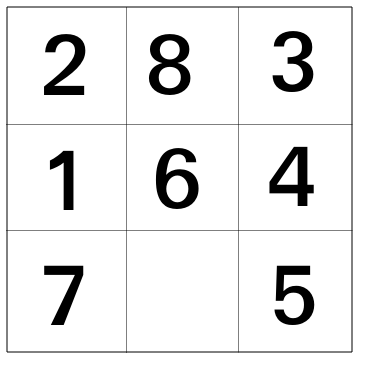
\includegraphics[width=4cm]{test1.png}}
  \caption{Тестовая начальная конфигурация 1}
  \label{fig:test1}
\end{figure}
\begin{figure}[H]
  \makebox[\textwidth][c]{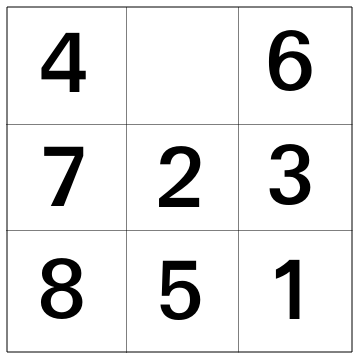
\includegraphics[width=4cm]{test2.png}}
  \caption{Тестовая начальная конфигурация 2}
  \label{fig:test2}
\end{figure}
\begin{figure}[H]
  \makebox[\textwidth][c]{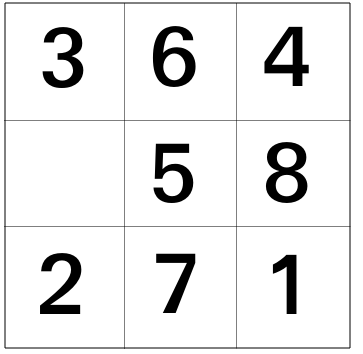
\includegraphics[width=4cm]{test3.png}}
  \caption{Тестовая начальная конфигурация 3}
  \label{fig:test3}
\end{figure}
Первая и третья начальные конфигурации имеют решения, т.к. количества
инверсий в соответствующих им перестановках нечетны. Вторая
конфигурация не имеет решения, т.к. количество инверсий для ее
перестановки четно.

В ходе тестирования были найдены решения конфигураций 1 и 2, для конфигурации 3 программа не смогла найти решения, как и было задумано. Решения для конфигураций 1 и 2, полученные с помощью программы, приводят к целевой конфигурации, что было проверено с помощью предиката solver и вручную.
\begin{figure}[H]
\[[moveUp, moveUp, moveLeft, moveDown, moveRight]\]
\caption{Решение для конфигурации 1}
\end{figure}
\begin{figure}[H]
  \begin{align*}
[moveDown, moveRight, moveUp, moveUp, moveRight, moveDown, moveDown,\\
  moveLeft, moveUp, moveRight, moveUp, moveLeft, moveLeft, moveDown,\\
  moveRight, moveRight, moveUp, moveLeft, moveLeft, moveDown,\\
  moveRight]
  \end{align*}
\caption{Решение для конфигурации 1}
\end{figure}

\section*{Вывод}
В ходе выполнения данной лабораторной работы я овладел методологией
решения логических задач с применением известных на сегодняшний день
стратегий поиска в пространстве состояний.
\end{document}
